% !TeX spellcheck = en_GB

% ------------------------------- %
%% Dataset, fitting, results %%
% ------------------------------- %

\begin{frame}{Fit AdaBoost}

%\hspace{-1em}
%\begin{figure}
%\subfloat{\includegraphics[width=0.5\paperwidth]{../r/plots/cv-adaboost.pdf}}
%\subfloat{\includegraphics[width=0.5\paperwidth]{../r/plots/adaboost-varimp.pdf}}
%\end{figure}

%$M_{\text{max}}=1000$, $\lambda=0.1$, $\pi=0.5$

%\texttt{ada::ada(<\emph{data}>, loss="exponential", type="discrete", nu=0.1, iter=1000, bag.frac=0.5)}

\begin{columns}[T]
\hspace{-2.3em}\begin{column}{0.515\textwidth}
	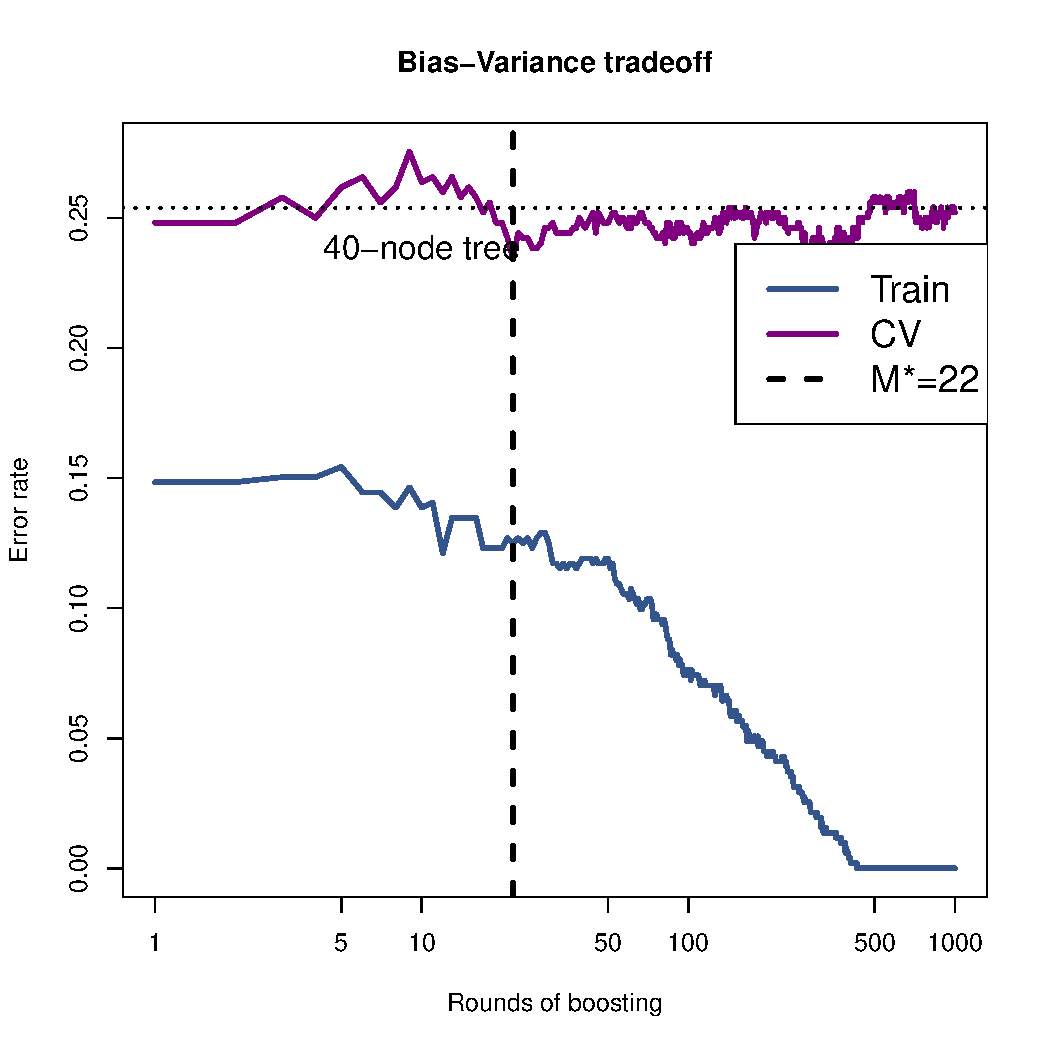
\includegraphics[width=1.21\columnwidth]{../r/plots/cv-adaboost-diab.pdf}
\end{column}
\hspace{-1.3ex}\begin{column}{0.515\textwidth}
	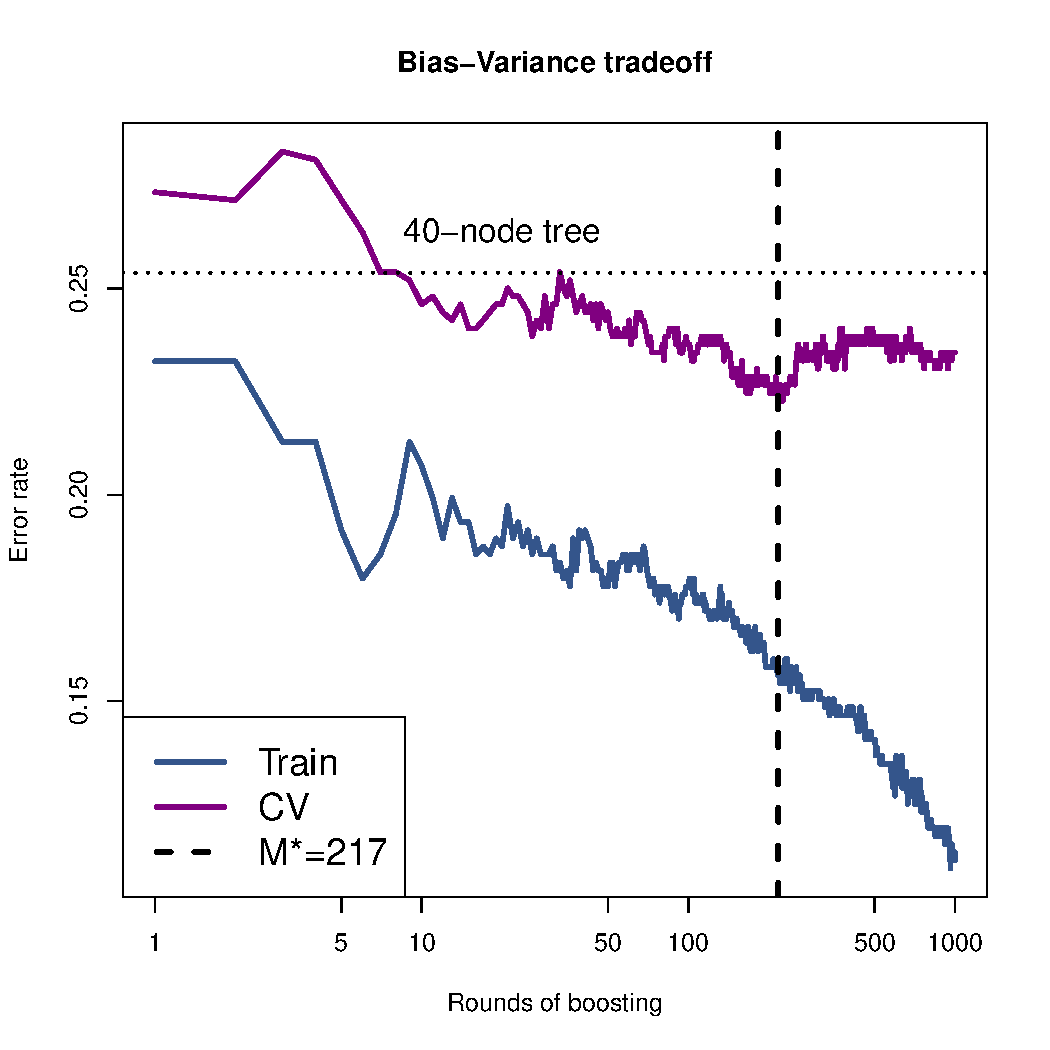
\includegraphics[width=1.21\columnwidth]{../r/plots/cv-adaboost-st-diab.pdf}
\end{column}
\end{columns}

\end{frame}

% col bagging ha bisogno di maggiori iterazioni prima di arricare all'overfitting (anche se nel boosting non si verifica effettivamente, è solo teorico)

%\begin{frame}{Fit AdaBoost (apple quality)}
%
%\begin{columns}[T]
%\hspace{-2.3em}\begin{column}{0.515\textwidth}
%	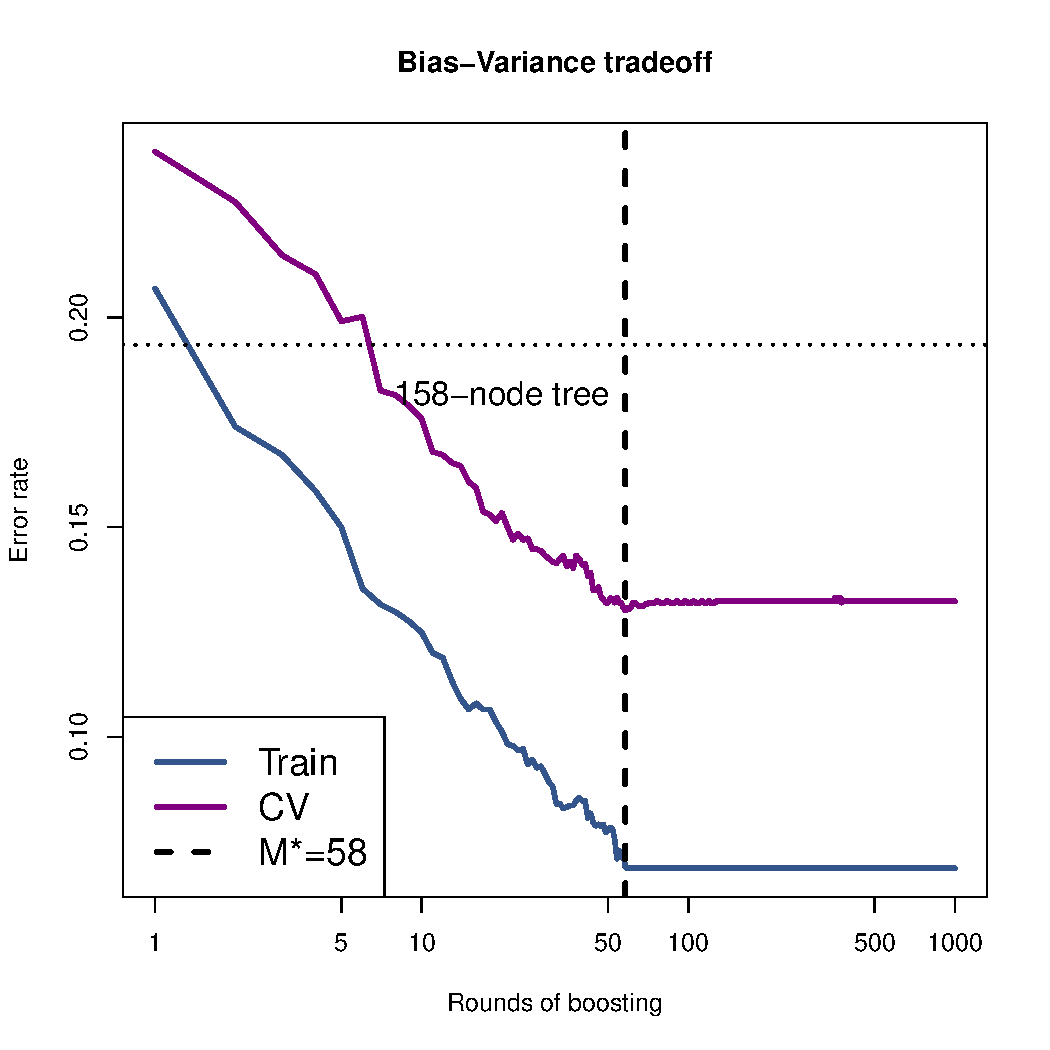
\includegraphics[width=1.21\columnwidth]{../r/plots/cv-adaboost-apple.pdf}
%\end{column}
%\hspace{-1.3ex}\begin{column}{0.515\textwidth}
%	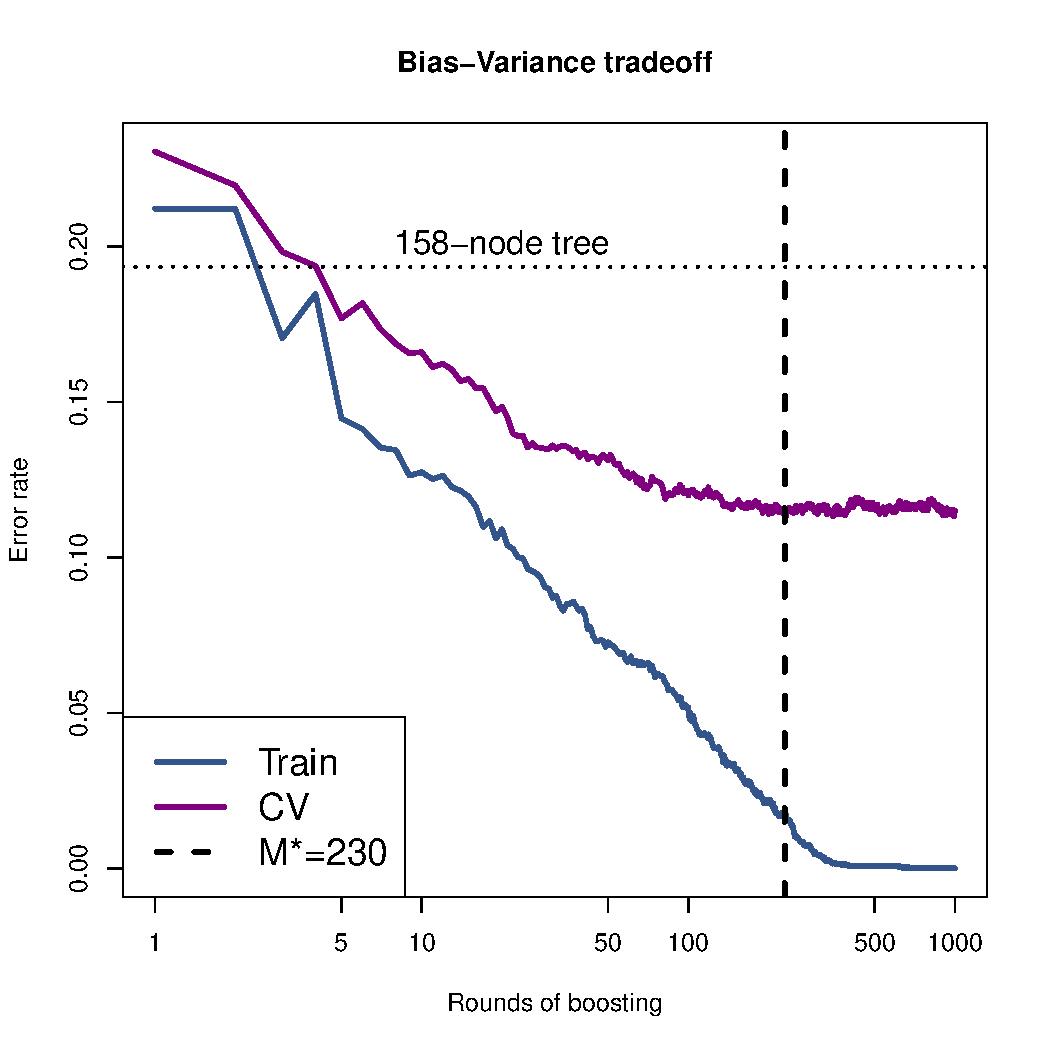
\includegraphics[width=1.21\columnwidth]{../r/plots/cv-adaboost-st-apple.pdf}
%\end{column}
%\end{columns}
%
%\end{frame}

% ------------------------------- %

%\begin{frame}{AdaBoost stochastic setting}

% a sinistra qualcosa di teoria (tipo il journey to the final classifier)
% a destra il bias-variance

%\vspace*{-0.5em}\begin{columns}[T]
%\begin{column}{0.48\textwidth}
%\begin{figure}
%\hspace{-2em}\begin{tikzpicture}
%	%draw,ellipse,fill=red!20,minimum height=2em,text centered,font=\sffamily\small
%	\tikzset{help lines/.append style=pink}
%%	\draw [help lines] (-2,-8) grid (3,1); \node[draw,circle,red] at (0,0) {};
%	
%	\node[cloud2] (m1) at (0,0) {$w^{(1)}, \pi_1$};
%	\node[cloud2] (m2) at (0,-1.25) {$w^{(2)}, \pi_2$};
%	\node[cloud2] (M) at (0,-4.5) {$w^{(M)}, \pi_M$};
%	\draw[-latex] (m1) to (m2);
%	\draw[-,dotted,very thick] ($(m2.south) + (0,-0.15)$) to ($(M.north) + (0,+0.15)$);
%	
%	\node (G1) at (2.3,0) {$G_1, f_1$};
%	\node (G2) at (2.3,-1.25) {$G_2, f_2$};
%	\node (GM) at (2.3,-4.5) {$G_M, f_M$};
%	\draw[-stealth] ($(m1.east) + (0.15,0)$) to (G1);
%	\draw[-stealth] ($(m2.east) + (0.15,0)$) to (G2);
%	%	\draw[-,dotted] (G2) to (GM);
%	\draw[-stealth] ($(M.east) + (0.15,0)$) to (GM);
%	
%	%	\node[rectangle,fill=pink!80] (G) at (1.5,-6) {$G(x)=\sign\Bigl(\sum_{m=1}^M\beta_mG_m(x)\Bigr)$};
%	\node[rectangle,fill=teal!20,font=\large,right] (f) at (-1,-5.55) {$L(y,f(x))=\exp(-yf(x))$};
%	\node[rectangle,fill=red!20,font=\large,right] (G) at (-1,-6.3) {$f_m(x)=f_{m-1}(x)+\lambda\alpha_mG_m(x)$};
%	\node[rectangle,fill=mLightGreen!20,font=\large,right] (L) at (-1,-7.05) {$G(x)=\sign(f_M(x))$};
%	%	\draw[-stealth] (GM) to (G);
%
%	\begingroup\linespread{0.9}
%	\node[font=\footnotesize,text width=4em,centered,text centered,inner sep=0pt] (pi) at (2.8,-2.6) {dataset random subsample};
%	\endgroup
%	\draw[-latex] (pi) to ($(m2.east) + (-0.25,-0.1)$);
%\end{tikzpicture}
%\end{figure}
%\end{column}
%\begin{column}{0.48\textwidth}
%\begin{figure}
%	\hspace*{-1.8em}\includegraphics[width=1.3\columnwidth]{../r/plots/cv-adaboost-st.pdf}
%\end{figure}
%$\pi=0.7$, $\lambda=0.1$
%% il learning rate basso viene compensato dal M* alto
%\end{column}
%\end{columns}
%
%\end{frame}



\begin{frame}{Variable importance}

\begin{columns}[T]
\hspace{-2.5em}\begin{column}{0.515\textwidth}
	% boosting setting
	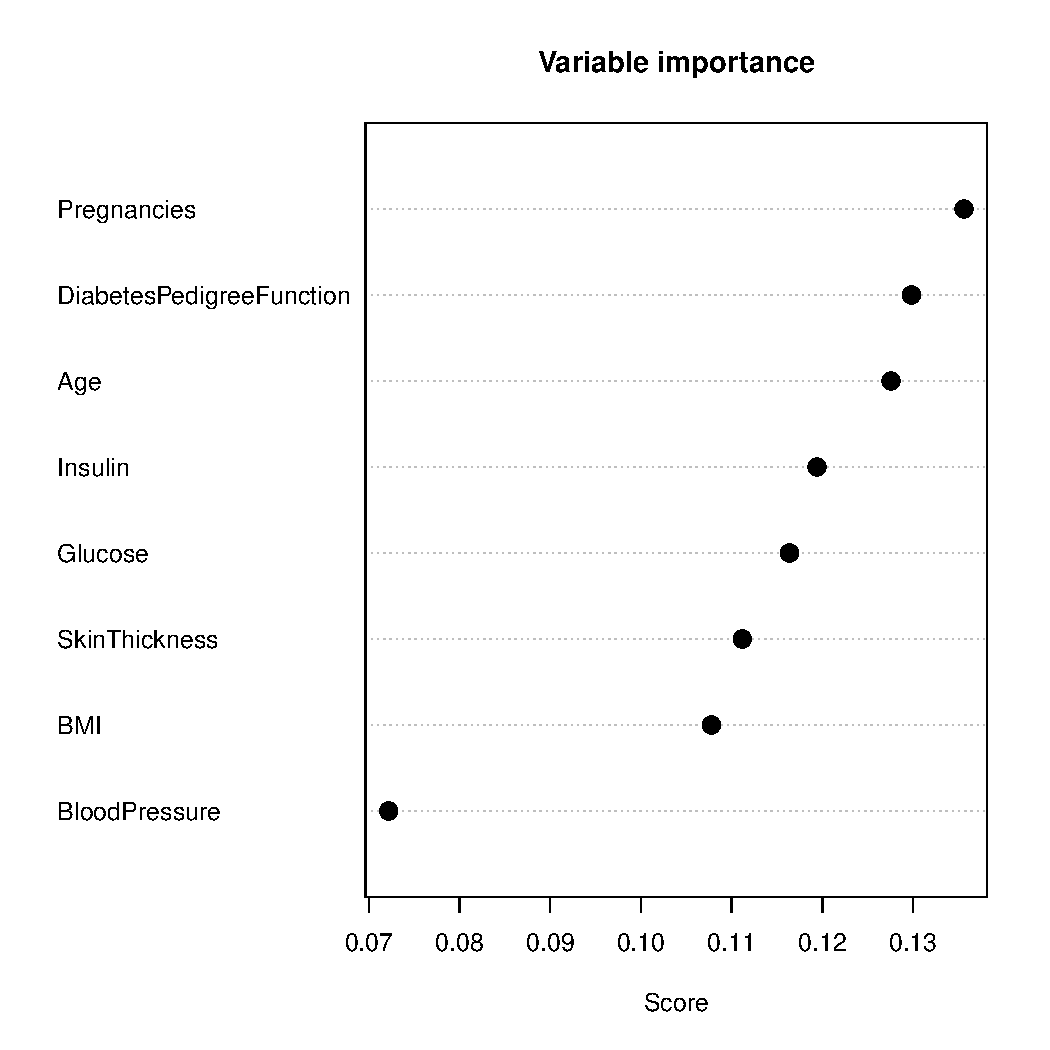
\includegraphics[width=1.21\columnwidth]{../r/plots/vip-adaboost-diab.pdf}
\end{column}
\hspace{-1.3ex}\begin{column}{0.515\textwidth}
	% stochastic setting
	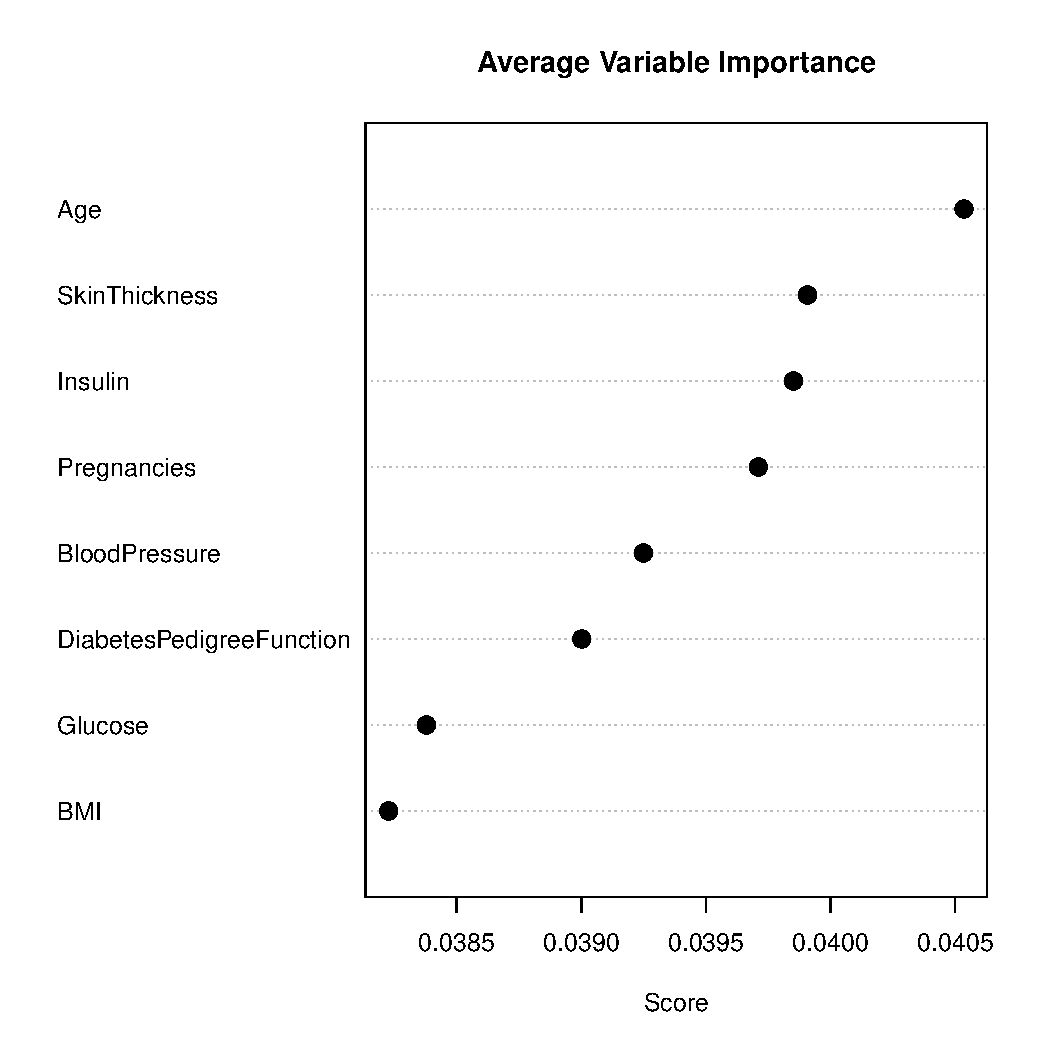
\includegraphics[width=1.21\columnwidth]{../r/plots/vip-adaboost-st1-diab.pdf}
\end{column}
\end{columns}

\end{frame}



%\begin{frame}{Variable importance (apple quality)}
%
%\begin{columns}[T]
%\hspace{-2.5em}\begin{column}{0.515\textwidth}
%	% boosting setting
%	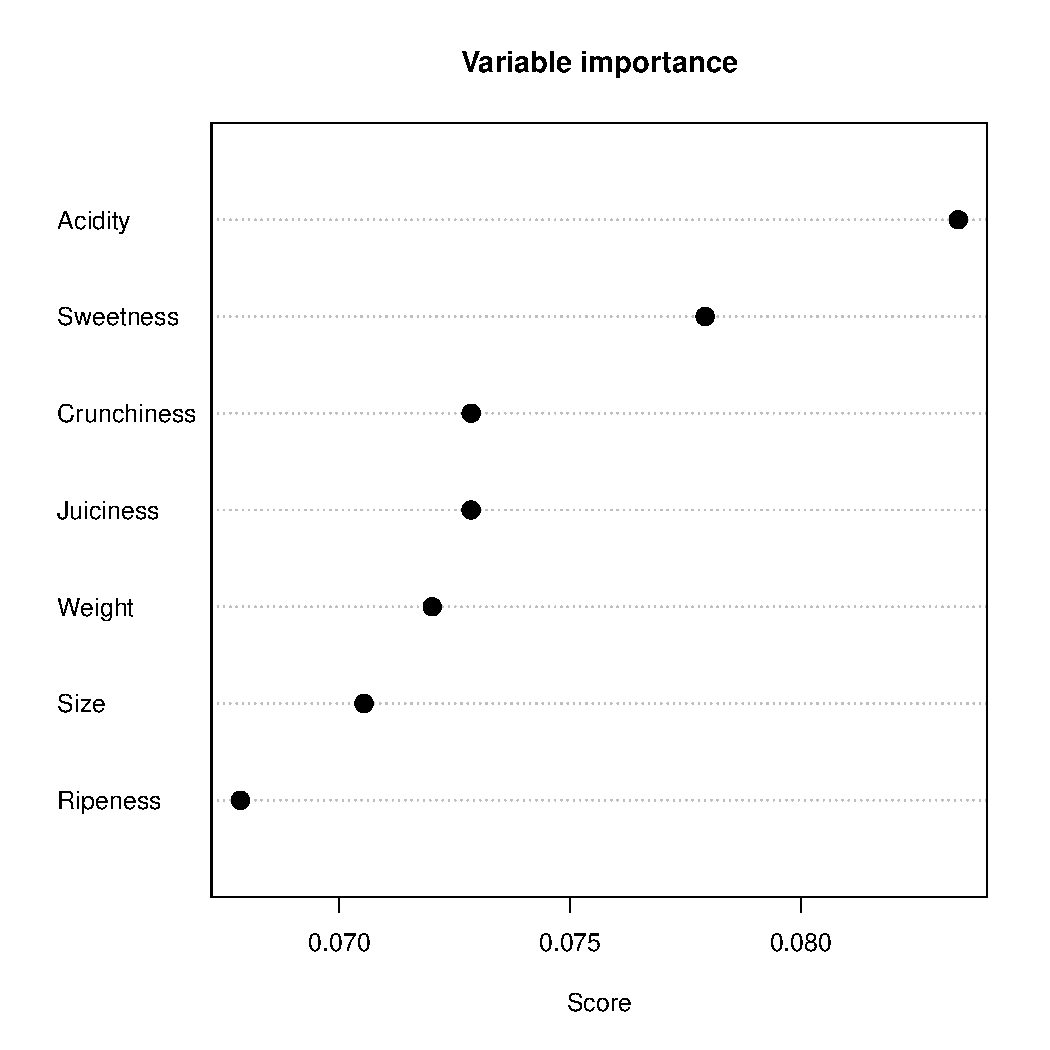
\includegraphics[width=1.21\columnwidth]{../r/plots/vip-adaboost-apple.pdf}
%\end{column}
%\hspace{-1.3ex}\begin{column}{0.515\textwidth}
%	% stochastic setting
%	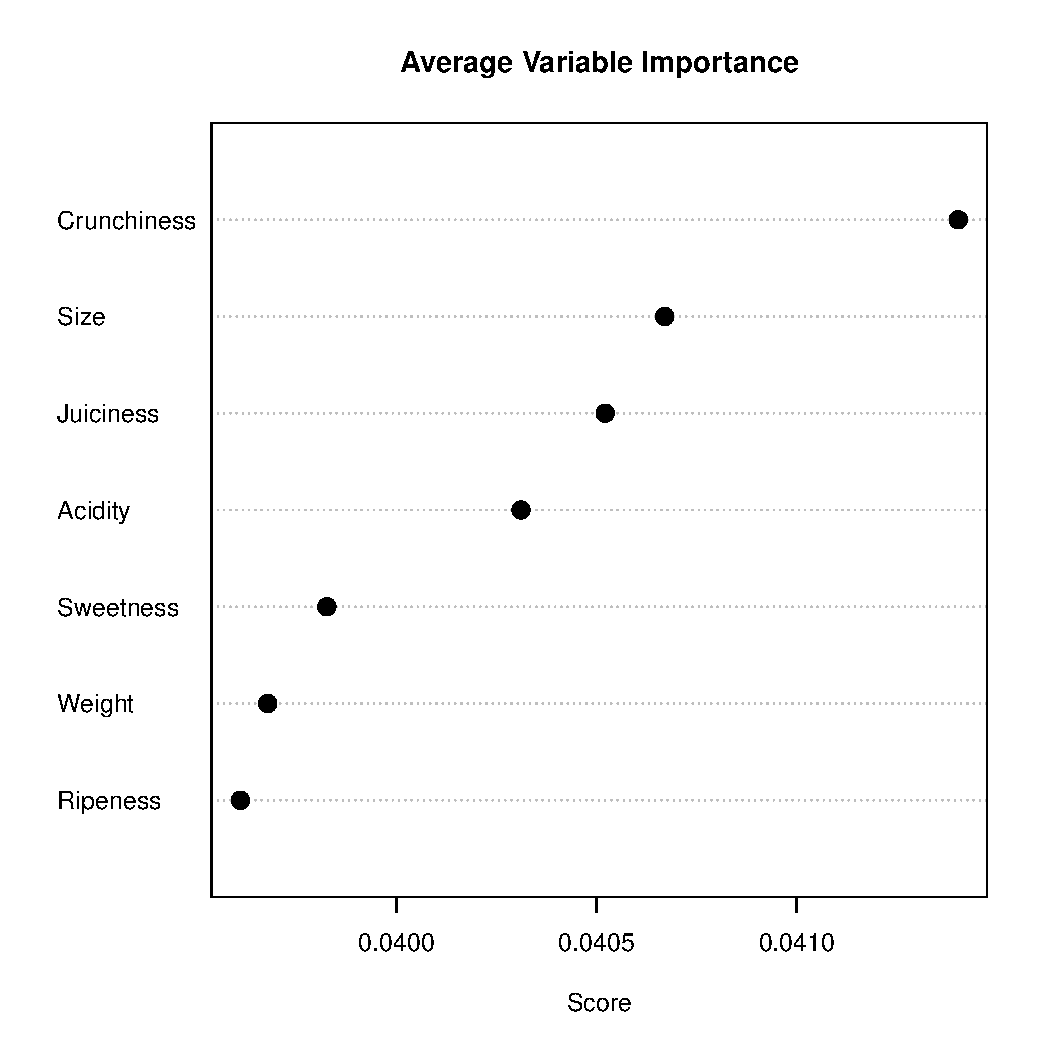
\includegraphics[width=1.21\columnwidth]{../r/plots/vip-adaboost-st1-apple.pdf}
%\end{column}
%\end{columns}
%
%\end{frame}



%\begin{frame}%{All models variable importance}
%
%% change plot title with model name
%% remove xlab (from R or just trim it)
%
%\vspace*{-0.5em}
%\begin{columns}[T]
%\hspace{1em}\begin{column}{0.515\textwidth}
%	% boosting setting
%	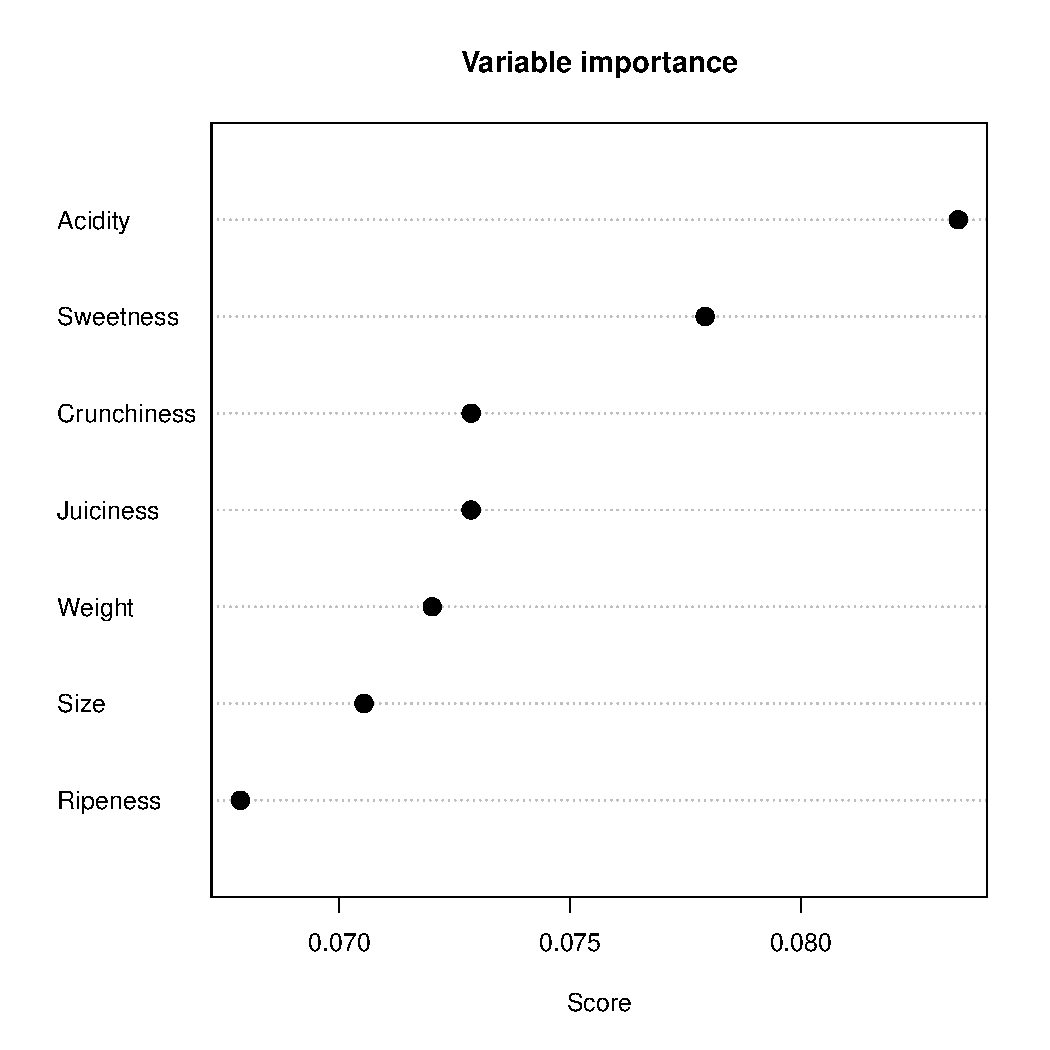
\includegraphics[width=0.9\columnwidth]{../r/plots/vip-adaboost-apple.pdf}\vspace{-1em}
%	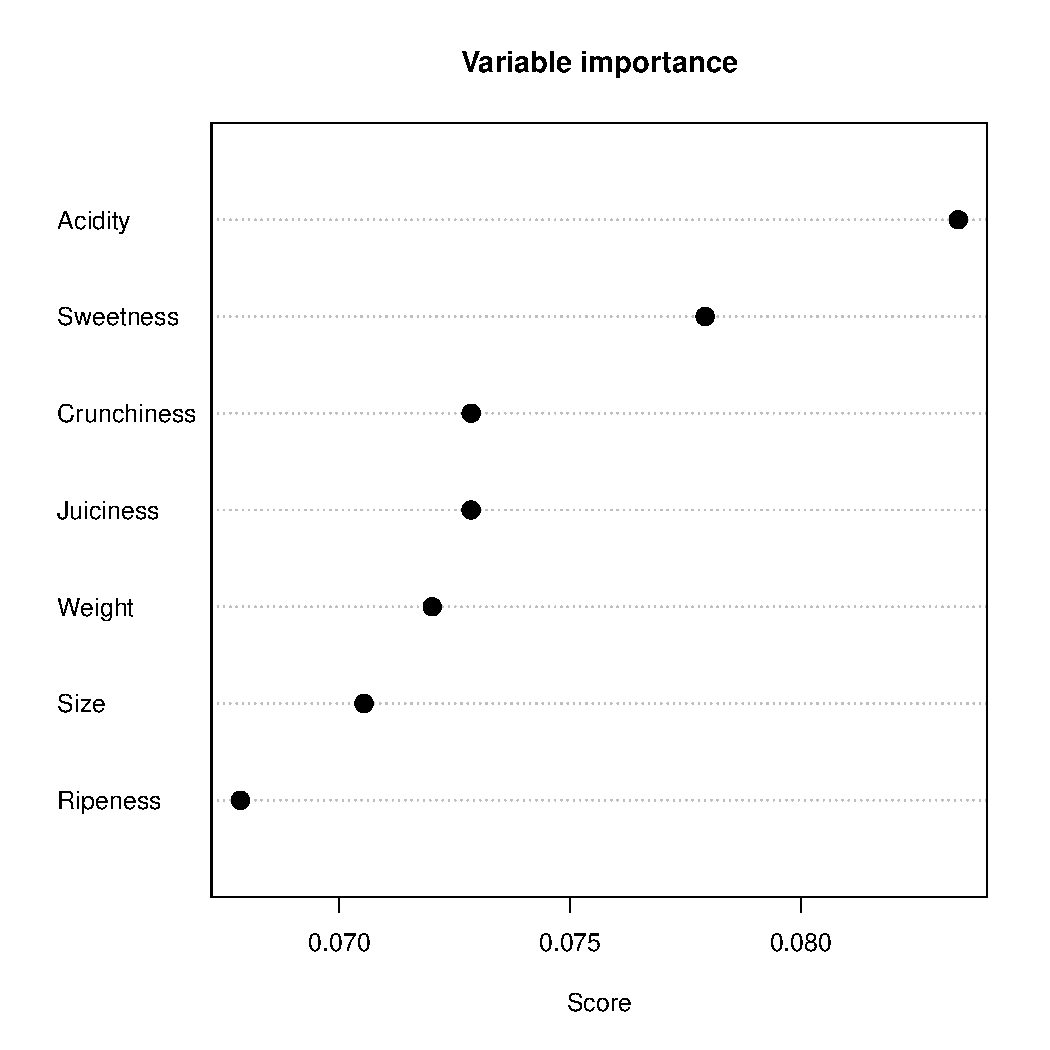
\includegraphics[width=0.9\columnwidth]{../r/plots/vip-adaboost-apple.pdf}
%\end{column}
%\hspace{-1.3ex}\begin{column}{0.515\textwidth}
%	% stochastic setting
%	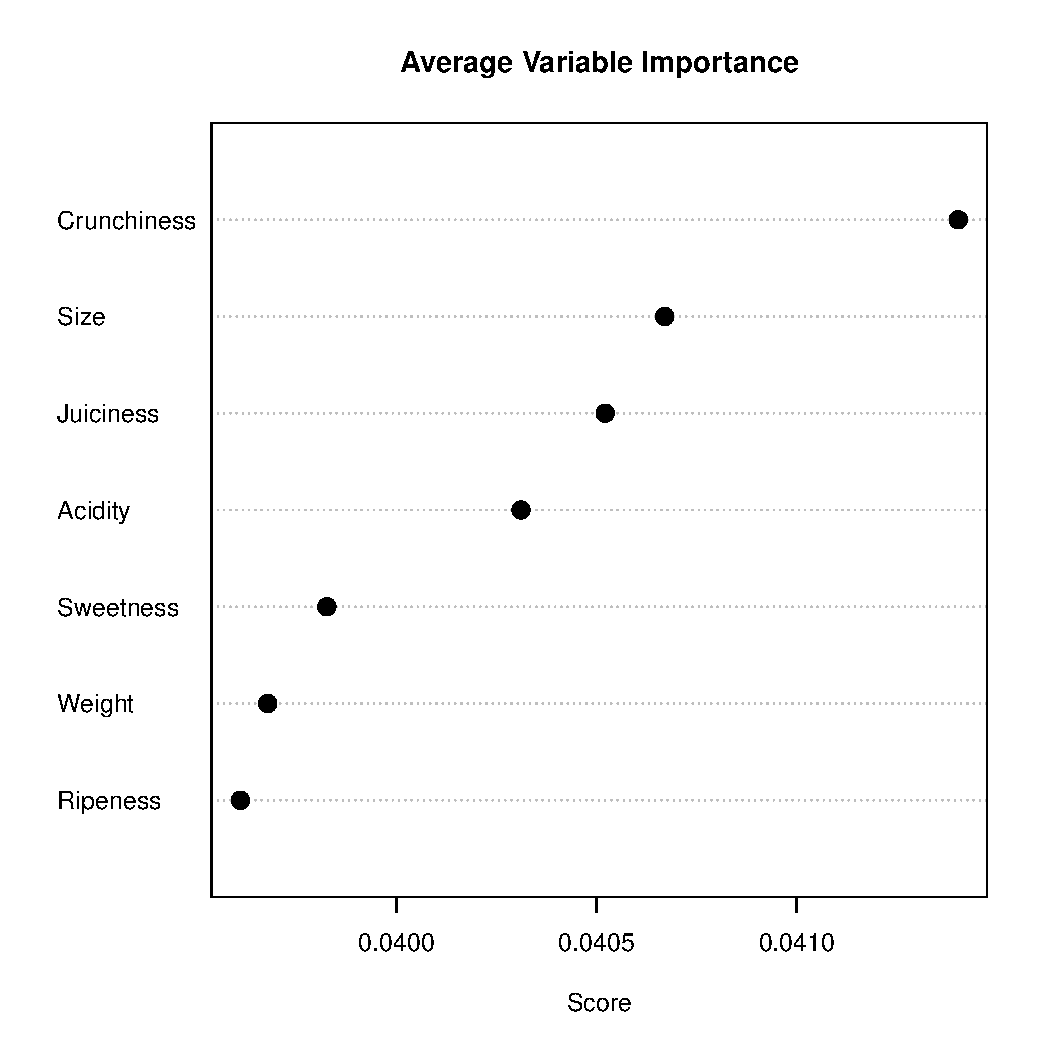
\includegraphics[width=0.9\columnwidth]{../r/plots/vip-adaboost-st1-apple.pdf}\vspace{-1em}
%	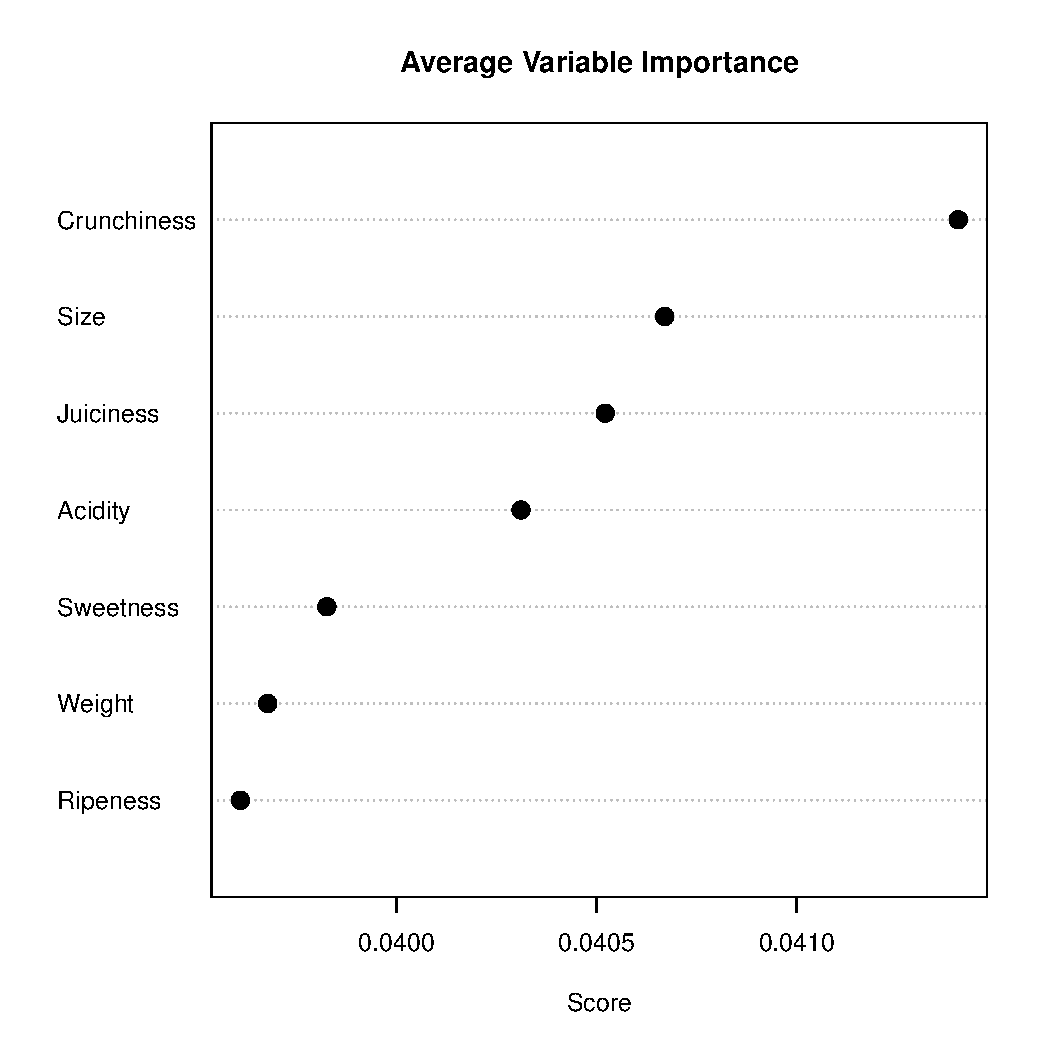
\includegraphics[width=0.9\columnwidth]{../r/plots/vip-adaboost-st1-apple.pdf}
%\end{column}
%\end{columns}
%
%\end{frame}

%\begin{frame}{Variable importance}
%
%\begin{figure}
%\hspace*{-3.2em}\begin{tikzpicture}
%%	\draw[help lines] (-5,-3) grid (6,3);\node[black,draw,circle] at (0,0) {};
%	% display anchors
%	\node[immagine] at (-5,-3) {\includegraphics[width=0.63\textwidth]{../r/plots/vip-adaboost-st0.pdf}};
%	\node[immagine,above left] at (8.2,-3) {\includegraphics[width=0.63\textwidth]{../r/plots/vip-adaboost-st1.pdf}};
%	
%	\draw[latex-latex,thick,bend left=10] (-3.4,2.4) to (1.6,-1.4);
%	\draw[latex-latex,thick,bend left=3] (-4.15,-1.4) to (1.6,1.8);
%
%	\node[draw,circle,thick,minimum size=0.4cm,mLightBrown] at (-4.48,-1.47) {};
%	\node[draw,circle,thick,minimum size=0.4cm,mLightBrown] at (1.92,1.88) {};
%
%	\node[draw,ellipse,thick,minimum width=1.2cm,mLightGreen] at (-4.1,2.45) {};
%	\node[draw,ellipse,thick,minimum width=1.2cm,mLightGreen] at (2.3,-1.45) {};
%\end{tikzpicture}
%\end{figure}
%
%\vspace{-1em}
%$M_{\text{max}}=1000$, $M^\ast=27$, $\lambda=1$, $\pi=0.5$
%
%\end{frame}

%\begin{frame}{Tuning}
%% error rate against rounds of boosting
%\begin{figure} % consider annotating M*
%\includegraphics[width=0.7\textwidth]{../r/plots/cv-adaboost.pdf}
%\end{figure}
%\end{frame}

%\begin{frame}{Variable importance}
%
%\begin{figure}
%\includegraphics[width=0.7\textwidth]{../r/plots/adaboost-varimp.pdf}
%\end{figure}
%
%\end{frame}
